\pagestyle{plain}
\selectlanguage{spanish}
\spanishdecimal{.}
\chapter*{Resumen}

\begin{flushleft}
  {\Large\bfseries Separación de señales electromiográficas según el músculo de procedencia\\[0.4cm]}

  \textbf{Autor:} Anton Cobian Iregui\\
  \textbf{Director:} Romano Giannetti\\
  \textbf{Entidad Colaboradora:} Universidad Pontificia Comillas, ICAI
\end{flushleft}
% ── Resumen breve ──────────────────────────────────────────
Este Trabajo Fin de Grado estudia la separación de señales EMG débiles mezcladas con
interferencias musculares más intensas en escenarios de músculos reinervados. Se comparan ICA, SOBI,
ICA restringido y regresión bajo condiciones controladas, mostrando que la recuperación depende de la mezcla, el retardo y la información previa.

\medskip
\noindent\textbf{Palabras clave:} 
Procesamiento de señal, EMG, Separación de fuentes, Prótesis
\bigskip

% ── Introducción ───────────────────────────────────────────
\section*{Introducción}

Este Trabajo Fin de Grado está motivado por un proyecto de investigación desarrollado en el Instituto de Investigación Tecnológica de la Universidad Pontificia Comillas, comúnmente conocido como IIT. El proyecto se centra en sistemas EMG implantables para ortesis mioeléctricas y reconstrucción biónica tras lesiones graves de nervios periféricos. En este contexto, las señales EMG se utilizan para estimar la intención de movimiento del usuario y traducirla en comandos de control para prótesis.

Sin embargo, en escenarios de músculos reinervados, la señal EMG medida puede verse afectada por atenuación, retardos temporales, patrones de activación atípicos y contaminación procedente de músculos donantes. Esto es especialmente relevante cuando la componente objetivo es más débil que la actividad muscular que interfiere, ya que la información deseada puede ser enmascarada por fuentes de mayor amplitud.

Por tanto, este trabajo estudia si las técnicas de separación de fuentes pueden ayudar a recuperar componentes EMG débiles a partir de las mezclas observadas. En lugar de reconstruir exactamente la forma de la señal original, el objetivo principal es preservar el patrón de activación de la fuente deseada, puesto que contiene la información más relevante para el control basado en EMG.
\clearpage
\section*{Definición del problema}

El problema específico que se aborda en este trabajo está inspirado en la interferencia que puede aparecer en sistemas VDMT (\textit{Vascularized Denervated Muscle Target}). En estos casos, el músculo reinervado puede generar una señal EMG débil, mientras que el músculo auxiliar puede introducir una contribución de mayor amplitud en el canal.

\begin{figure}[H]
  \centering
 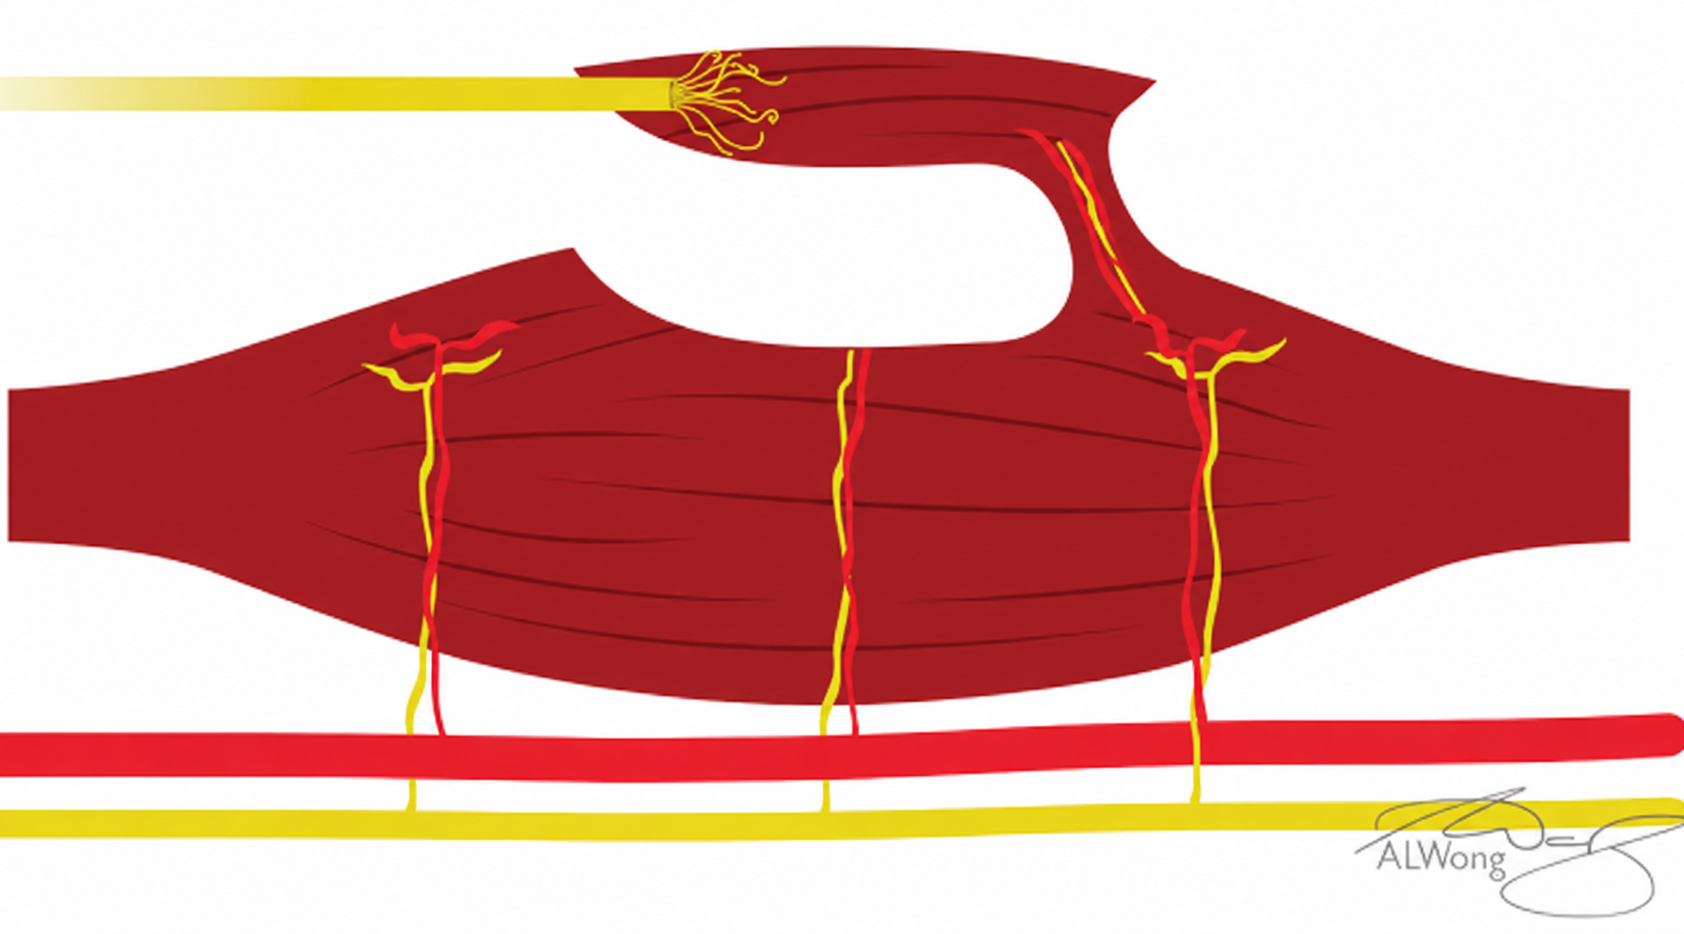
\includegraphics[width=0.8\textwidth]{figuras/introduction/VDMT_diagram_modified.png}
  \caption{Ilustración esquemática de un VDMT, adaptada de \cite{tuffaha_vascularized_2020}.}
  \label{fig:resumen_vdmt}
\end{figure}

Por ello, el problema de separación se modela como un sistema de dos fuentes y dos canales. La fuente objetivo se expresa como $s_1$, mientras que la fuente de interferencia de mayor amplitud se denomina $s_2$. Aunque a lo largo del trabajo se consideran varios modelos para analizar el efecto de la interferencia, el ruido y el retardo, el caso del estudio del IIT se modela como un escenario asimétrico con una fuente débil, como se describe en la Ecuación \ref{eq:resumen_modelo}.

\begin{equation}
    \left\{
\begin{aligned}
c_1(t) &= s_1(t) + \beta s_2(t-\tau) + n_1(t) \\
c_2(t) &= 0.01 s_1(t-\tau) + s_2(t) + n_2(t) 
\end{aligned}
\right.
\label{eq:resumen_modelo}
\end{equation}
\\
\noindent donde $\beta$ representa el factor de interferencia en la fuente débil, $\tau$ el retardo temporal entre canales y $n_1(t), n_2(t)$ ruido aditivo con varianza $\sigma^2$.

El modelo describe una mezcla asimétrica en la que la señal objetivo débil está fuertemente contaminada por el músculo auxiliar, mientras que el canal del donante contiene una contribución mínima de dicha señal. Por este motivo, el objetivo es estimar la fuente débil $s_1$ a partir de las mezclas observadas y obtener una estimación $\hat{s}_1$ que mantenga sus patrones de activación.
\section*{Metodología}

La metodología experimental se estructura en varias etapas. Dado que todavía no se dispone de datos experimentales específicos de sistemas VDMT, las pruebas se realizan con señales EMG procedentes de una base de datos de pacientes con TMR (otra técnica de reinervación muscular). Estas señales se emplean como base experimental, junto con señales artificiales diseñadas para simular diferentes frecuencias de activación. A continuación, las señales seleccionadas se adaptan y se mezclan mediante los modelos propuestos con el fin de simular distintos niveles de interferencia, ruido y retardo.

Antes de aplicar los algoritmos de separación, las señales se preprocesan mediante filtrado, escalado de canales y blanqueamiento. El filtrado reduce componentes espectrales no deseadas, el escalado mejora la comparabilidad entre canales y el blanqueamiento prepara los datos para la etapa de separación.

Posteriormente, se implementan y comparan varios métodos. FastICA se utiliza como el principal algoritmo de separación ciega basado en la no gaussianidad. SOBI se estudia como un método alternativo basado en la correlación temporal. ICA restringido se propone para evaluar si la información previa puede guiar la separación hacia la fuente deseada. Finalmente, la regresión lineal se considera cuando uno de los canales puede aproximarse a la fuente de interferencia.

Los resultados se evalúan mediante la correlación con la envolvente RMS, la correlación temporal y la SNR. Entre estas métricas, se prioriza la correlación con la envolvente RMS, ya que el control de prótesis mediante EMG depende principalmente de la detección del patrón de activación. En este contexto, la reconstrucción exacta de la onda original tiene una importancia secundaria. El flujo experimental se resume en la Figura \ref{fig:methodoloy_pipeline2}.
\\
\begin{figure}[H]
    \centering
    \makebox[\textwidth][c]{%
    \resizebox{1.25\textwidth}{!}{%
    \begin{tikzpicture}[
        block/.style={
            draw,
            rectangle,
            minimum width=3.4cm,
            minimum height=2cm,
            text width=2.7cm,
            align=center,
            font=\small
        },
        arrow/.style={-{Stealth}, thick},
        label/.style={font=\small, above}
    ]

    \node[block] (sig) {Selección\\y adaptación\\de señales};
    \node[block, right=1.2cm of sig] (mix) {Modelo\\de mezcla};
    \node[block, right=1.2cm of mix] (pre) {Preprocesamiento};
    \node[block, right=1.2cm of pre] (sep) {Algoritmo\\de separación};
    \node[block, right=1.2cm of sep] (ass) {Evaluación};

    \draw[arrow] (sig.east) -- node[label]{$s_1, s_2$} (mix.west);
    \draw[arrow] (mix.east) -- node[label]{$c_1, c_2$} (pre.west);
    \draw[arrow] (pre.east) -- node[label]{$z_1, z_2$} (sep.west);
    \draw[arrow] (sep.east) -- node[label]{$\hat{s}_1, \hat{s}_2$} (ass.west);

    \end{tikzpicture}
    }%
    }
    \caption{Diagrama de bloques del proceso seguido en los experimentos de este trabajo.}
    \label{fig:methodoloy_pipeline2}
\end{figure}

\section*{Resultados}

Los resultados muestran que ICA funciona adecuadamente en mezclas instantáneas ideales o casi ideales, recuperando las fuentes con las indeterminaciones de orden, signo y escala. Con ruido aditivo, la correlación temporal de la fuente débil disminuye, pero su envolvente RMS se preserva en algunos casos.

Sin embargo, el rendimiento de ICA empeora cuando se introducen retardos temporales. Esto se debe a que una matriz de separación instantánea no puede cancelar completamente las contribuciones retardadas de la fuente dominante. Esto afecta principalmente a la recuperación de la componente débil, especialmente cuando la fuente de interferencia presenta una varianza mucho mayor.

SOBI no proporciona una mejora consistente frente a ICA para las señales EMG reales consideradas, ya que sus patrones de autocorrelación suelen ser demasiado similares. ICA restringido ofrece un marco flexible usando información previa, pero las referencias binarias evaluadas en este trabajo no muestran una mejora significativa. La regresión con retardo muestra los mejores resultados únicamente si $c_2$ es una referencia fiable de $s_2$ y el retardo puede estimarse con precisión. Esto sugiere que las técnicas convolutivas podrían hacer frente a la contribución retardada de $s_2$, una de las principales limitaciones de los métodos instantáneos estudiados en este trabajo.

\begin{figure}[H]
  \centering
   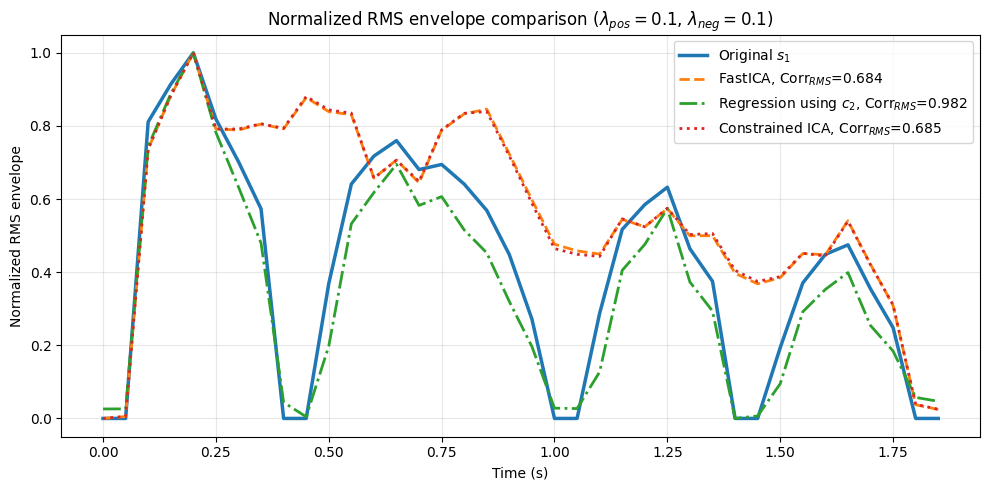
\includegraphics[width=\textwidth]{figuras/constrained/comparison_beta_05_tau_5_with_delayed_regression.png}
  \caption{Comparación de las envolventes RMS recuperadas por los algoritmos. Los parámetros se fijaron a $\sigma=0.1$, $\beta=0.3$ y $\tau=\qty{5}{ms}$. La regresión con retardo logra una reconstrucción casi perfecta ya que elimina la interferencia retardada procedente de $s_2$.}
  \label{fig:resultados_resumen}
\end{figure}

\section*{Conclusiones}

Este trabajo muestra que los métodos de separación de fuentes pueden ser útiles para recuperar componentes EMG débiles, pero su rendimiento depende fuertemente de las condiciones de mezcla. En particular, los retardos temporales, el ruido aditivo y la dominancia de una fuente dificultan significativamente la recuperación de la señal deseada.

La principal conclusión es que la recuperación de una fuente débil no siempre puede resolverse mediante separación ciega e instantánea. Cuando la mezcla se aproxima al caso ideal, los métodos estándar de BSS pueden proporcionar buenos resultados, pero el escenario del IIT introduce información adicional que debería aprovecharse. En concreto, la presencia de un canal de referencia y la estimación del retardo temporal son factores clave en la recuperación del patrón de activación.

En conjunto, los resultados sugieren que recuperar actividad EMG débil en escenarios de músculos reinervados puede requerir más que separación ciega estándar. El trabajo futuro debería centrarse en una mejor estimación del retardo con modelos convolutivos, restricciones fisiológicas significativas, señales EMG multicanal y validación con datos experimentales procedentes del proyecto del IIT.